% !TEX encoding = UTF-8 Unicode

\documentclass[a4paper]{article}

\usepackage{float}
\usepackage{color}
\usepackage{url}
\usepackage[T2A]{fontenc} % enable Cyrillic fonts
\usepackage[utf8]{inputenc} % make weird characters work
\usepackage{graphicx}

\usepackage[english,serbian]{babel}

\usepackage[unicode]{hyperref}
\hypersetup{colorlinks,citecolor=green,filecolor=green,linkcolor=blue,urlcolor=blue}

\newtheorem{primer}{Primer}[section]
\newcommand\todo[1]{\textcolor{red}{#1}}

\begin{document}

\title{Kako i zašto funkcioniše blockchain?\\ \small{Seminarski rad u okviru kursa\\Tehničko i naučno pisanje\\ Matematički fakultet}}
\author{
    Lazić, Jovana\\ 
    \texttt{kontakt email adresa autora}
    \and
    Nikić, Ognjen\\ 
    \texttt{kontakt email adresa autora}
    \and
    Nešković, Ognjen\\ 
    \texttt{mi22009@alas.matf.bg.ac.rs}
    \and
    Sekešan, Pavle\\ 
    \texttt{kontakt email adresa autora}
}
\date{\today}
\maketitle

\abstract{
U radu su sažeto iznete osnove kriptografije potrebne za razumevanje i implementaciju blokčejna. Ukratko je predstavljena istorija blokčejna, kao i glavne ideje potrebne za realizaciju blokčejna koji se nalazi iza jedne od najpoznatijih kriptovaluta - Bitcoin. \todo{Dopuniti kasnije...}
\tableofcontents

\newpage

\section{Uvod}
\label{sec:uvod}
\todo{Napisati uvod - ukratko nešto o istoriji blokčejna, čemu služi, zašto je koristan, pomenuti osnovne ideje koje se koriste (heširanje, merkle stabla, asimetrična kriptografija (digitalni potpisi) itd.)}

\section{Kriptografske osnove}	
\label{sec:kriptografske_osnove}

\subsection{Kriptografske heš funkcije}
\todo{Napisati ovaj subsection}

\subsection{Asimetrična kriptografija}
\todo{Napisati ovaj subsection}

\section{Blokčejn}
\label{sec:blockchain}

Blokčejn je decentralizovan, distribuiran i najčešće javan skup podataka (najčešće transakcija ili drugih zapisa) \cite{wood2014ethereum} sačinjen od manjih jedinica podataka - ''blokova''.
Blokovi su takvi da se dati blok ne može izmeniti bez promene svih blokova koji dolaze nakon njega. Ovim blokovi uspostavljaju ''istoriju'', odnosno sekvencu izmena na javnom skupu podataka.
\begin{figure}[H]
    \centering
        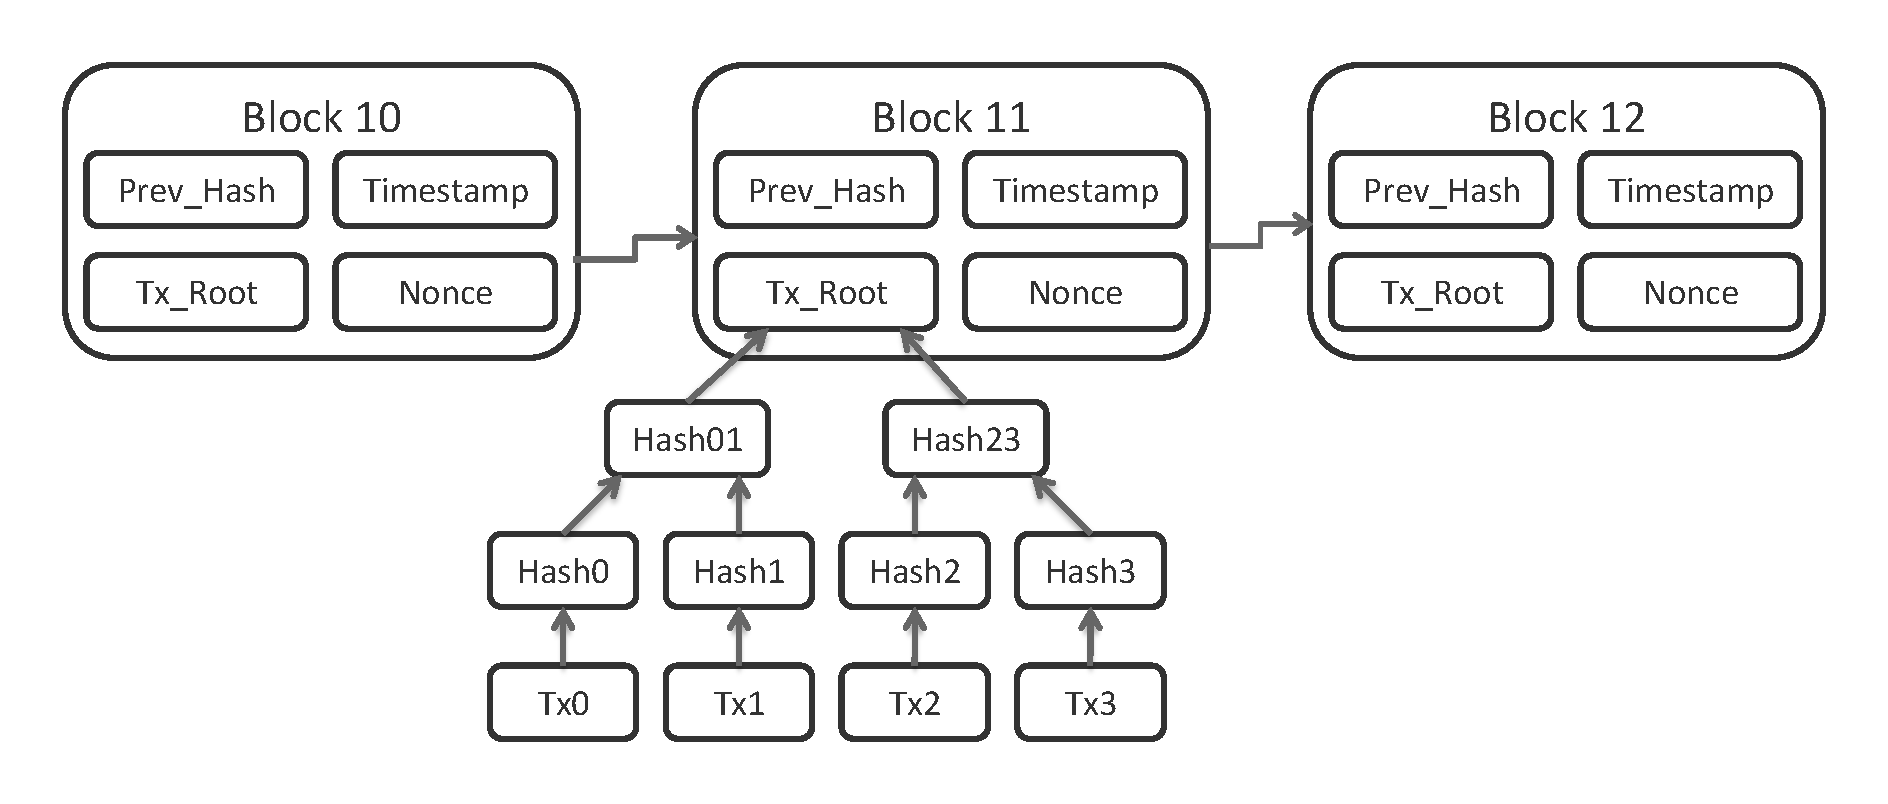
\includegraphics[scale=0.3]{bitcoin_blockchain_diagram.pdf}
    \caption{Bitcoin blokčejn}
    \label{fig:btc_blockchain}
\end{figure}
Na primer u slučaju Bitcoin blokčejna (slika \ref{fig:btc_blockchain}) blokovi sadrže, pored ostalog, heš prethodnog bloka i transakcije (preciznije merkle stablo izgrađeno nad transakcijama).
Time što jedan blok sadrži heš bloka koji je kreiran pre njega je uspostavljen redosled blokova, pa i time redosled transakcija.
Neke izmene nad skupom podataka moraju biti odobrene od strane pojedinca kome podaci pripadaju (na primer u slučaju transakcija) što se postiže metodama asimetrične kriptografije.
Svi učesnici u distribuiranoj mreži mogu lako verifikovati da li su izmene u blokčejnu validne i složiti se sa izmenama ili glasati protiv njih.
Kako bi se došlo do konsenzusa oko toga koja sekvenca izmena na blokčejnu je validna uvode se metode poput dokaza o izvršenom radu (proof of work), dokaza o posedovanju valute (proof of stake) itd.
Metode za postizanje konsenzusa se biraju tako da se postigne veliki stepen otpornosti prema ne-kooperativnim agentima u distribuiranoj mreži.
Zajedno sa javno dostupnim blokčejnom ovaj sistem rešava jedan od značajnih problema digitalnih dobara poznat kao ''double spending''. \cite{nakamoto2008bitcoin}


\subsection{Blokovi}
\todo{Napisati ovaj subsection - apstraktnije opisati pojam bloka u blokčejnu generalno (ne samo kod bitkojna), način za postizanje konsenzusa (proof of work, proof of stake,...), forkovi}

\subsection{Decentralizacija}
\todo{Napisati ovaj subsection - opisati kako blokčejn koristi peer to peer mrežu, sa konkretnim primerom (na primer kako bitkojn radi broadcast ili šta već), prednosti i mane decentralizacije generalno - double spending ako neko ima preko 51\%, itd. }

\section{Primene}
\label{sec:primene}

\subsection{Kriptovalute}
\todo{Napisati ovaj subsection}

\subsection{Pametni ugovori}
\todo{Napisati ovaj subsection - pomenuti eth pošto btc nije turing complete}

\section{Zaključak}
\todo{Napisati ovaj subsection}

\addcontentsline{toc}{section}{Literatura}
\appendix


\bibliography{seminarski} 
\bibliographystyle{plain}



\end{document}
